%%%%%%%%%%%%%%%%%%%%%%%%%%%%%%%%%%%%%%%%%
% McMaster Masters/Doctoral Thesis 
% LaTeX Template
% Version 2.2 (11/23/15)
%
% This template has been downloaded from:
% http://www.LaTeXTemplates.com
% Then subsequently from http://www.overleaf.com
%
% Version 2.0 major modifications by:
% Vel (vel@latextemplates.com)
%
% Original authors:
% Steven Gunn  (http://users.ecs.soton.ac.uk/srg/softwaretools/document/templates/)
% Sunil Patel (http://www.sunilpatel.co.uk/thesis-template/)
%
% Modified to McMaster format by Benjamin Furman (contact: https://www.xenben/com; Most up 
% to date template at https://github.com/benjaminfurman/McMaster_Thesis_Template, 
% occasionally updated on Overleaf template page)
%
% License:
% CC BY-NC-SA 3.0 (http://creativecommons.org/licenses/by-nc-sa/3.0/)
%
%%%%%%%%%%%%%%%%%%%%%%%%%%%%%%%%%%%%%%%%%

%----------------------------------------------------------------------------------------
% DOCUMENT CONFIGURATIONS
%----------------------------------------------------------------------------------------

\documentclass[
12pt, % The default document font size, options: 10pt, 11pt, 12pt
oneside, % Two side (alternating margins) for binding by default, uncomment to switch to one side
english, % other languages available
onehalfpacing, % Single line spacing, alternatives: onehalfspacing or doublespacing
%draft, % Uncomment to enable draft mode (no pictures, no links, overfull hboxes indicated)
%nolistspacing, % If the document is onehalfspacing or doublespacing, uncomment this to set spacing in lists to single
%liststotoc, % Uncomment to add the list of figures/tables/etc to the table of contents
%toctotoc, % Uncomment to add the main table of contents to the table of contents
]{McMasterThesis} % The class file specifying the document structure


%----------------------------------------------------------------------------------------
% Import packages here
%----------------------------------------------------------------------------------------
\usepackage[utf8]{inputenc} % Required for inputting international characters
\usepackage[T1]{fontenc} % Output font encoding for international characters

\usepackage{lmodern} % could change font type by calling a different package
\usepackage{lastpage} % count pages
\usepackage{siunitx} % for scientific units (micro-liter, etc)
\setcounter{tocdepth}{2} % so that only section and sub sections appear in Table of Contents. Remove or set depth to 3 to include sub-sub-sections

%----------------------------------------------------------------------------------------
% Handling Citations
%----------------------------------------------------------------------------------------
\usepackage[backend=biber, giveninits=true, doi=false, natbib=true, url=false, eprint=false, style=authoryear, sorting=nyt, maxcitenames=2, maxbibnames=99, uniquename=false, uniquelist=false, dashed=false]{biblatex} % can change the maxbibnames to cut long author lists to specified length followed by et al., currently set to 99.
\DeclareFieldFormat[article,inbook,incollection,inproceedings,patent,thesis,unpublished]{title}{#1\isdot} % removes quotes around title
\renewbibmacro*{volume+number+eid}{%
  \printfield{volume}%
%  \setunit*{\adddot}% DELETED
  \printfield{number}%
  \setunit{\space}%
  \printfield{eid}}
\DeclareFieldFormat[article]{number}{\mkbibparens{#1}}
%\renewcommand*{\newunitpunct}{\space} % remove period after date, but I like it. 
\renewbibmacro{in:}{\ifentrytype{article}{}{\printtext{\bibstring{in}\intitlepunct}}} % this remove the "In: Journal Name" from articles in the bibliography, which happens with the ynt 
\renewbibmacro*{note+pages}{%
    \printfield{note}%
    \setunit{,\space}% could add punctuation here for after volume
    \printfield{pages}%
    \newunit}    
\DefineBibliographyStrings{english}{% clears the pp from pages
  page = {\ifbibliography{}{\adddot}},
  pages = {\ifbibliography{}{\adddot}},
} 
\DeclareNameAlias{sortname}{last-first}
\renewcommand*{\nameyeardelim}{\addspace} % remove comma in text between name and date
\addbibresource{Bibliography.bib} % The filename of the bibliography
\usepackage[autostyle=true]{csquotes} % Required to generate language-dependent quotes in the bibliography

% you'll have to play with the citation styles to resemble the standard in your field, or just leave them as is here. 
% or, if there is a bst file you like, just get rid of all this biblatex stuff and go back to bibtex. 

%----------------------------------------------------------------------------------------
% Collect all your header information from the chapters here, things like acronyms, custom commands, necessary packages, etc. 
%----------------------------------------------------------------------------------------
\usepackage{parskip} %this will put spaces between paragraphs
\setlength{\parindent}{15pt} % this will create and indent on all but the first paragraph of each section. 
% should maybe change to glossaries package
\usepackage{acro}
\DeclareAcronym{est}{
	short = EST,
	long  = expressed sequence tags
}

\DeclareAcronym{Xl}{
	short = \textit{X.~laevis},
	long  = \textit{Xenopus~laevis}
}
\DeclareAcronym{Xg}{
	short = \textit{X.~gilli},
	long  = \textit{Xenopus~gilli}
}

\usepackage{etoolbox}
\preto\chapter{\acresetall} % resets acronyms for each chapter

\usepackage{xspace} %helps spacing with custom commands. 
\newcommand{\oddname}{{\sc SoME goOfY LonG ThiNg With an AwkWarD NAme}\xspace}


\usepackage{pgfplotstable} % a much better way to handle tables
\pgfplotsset{compat=1.12}

% \usepackage{float} % if you need to demand figure/table placement, then this will allow you to use [H], which demands a figure placement. Beware, making LaTeX do things it doesn't want may lead to oddities.  


%%%%
% LINK COLORS
% You can control the link colors at the end of the McMasterThesis.cls file. There is also a true/false option there to turn off all link colors.  
%%%%


%----------------------------------------------------------------------------------------
%	THESIS INFORMATION
%----------------------------------------------------------------------------------------

\thesistitle{Breast Cancer Specimen Classification} % Your thesis title, print it elsewhere with \ttitle
\supervisor{Dr. Nedialkov \textsc{Ned}} % Your supervisor's name, print it elsewhere with \supname
\examiner{} % Your examiner's name, print it elsewhere with \examname
\degree{Master of Engineering} % Your degree name, print it elsewhere with \degreename
\author{Shuo \textsc{Hou}} % Your name, print it elsewhere with \authorname
\addresses{} % Your address, print it elsewhere with \addressname

\subject{Computing & Software} % Your subject area, print it elsewhere with \subjectname
\keywords{} % Keywords for your thesis, print it elsewhere with \keywordnames
\university{\href{http://www.mcmaster.ca/}{McMaster University}} % Your university's name and URL, print it elsewhere with \univname
\department{\href{https://www.eng.mcmaster.ca/cas}{Department of Computing and Software}} % Your department's name and URL, print it elsewhere with \deptname
\group{\href{http://researchgroup.university.com}{Research Group Name}} % Your research group's name and URL, print it elsewhere with \groupname
\faculty{\href{https://www.eng.mcmaster.ca}{Faculty of Engineering}} % Your faculty's name and URL, print it elsewhere with \facname

% this sets up hyperlinks
\hypersetup{pdftitle=\ttitle} % Set the PDF's title to your title
\hypersetup{pdfauthor=\authorname} % Set the PDF's author to your name
\hypersetup{pdfkeywords=\keywordnames} % Set the PDF's keywords to your keywords

\begin{document}

 \frontmatter % Use roman page numbering style (i, ii, iii, iv...) for the pre-content pages

\pagestyle{plain} % Default to the plain heading style until the thesis style is called for the body content

%----------------------------------------------------------------------------------------
%	Half Title (lay title)
%----------------------------------------------------------------------------------------
%\begin{halftitle} % could not get this environment working
%\vspace*{\fill}
\vspace{6cm}
\begin{center}
A short 60 character title % ideally, but it doesn't seem to matter
\end{center}
%\vspace*{\fill}
\pagenumbering{gobble} % leave this here, McMaster doesn't want this page numbered
%\end{halftitle}
\clearpage

%----------------------------------------------------------------------------------------
%	TITLE PAGE
%----------------------------------------------------------------------------------------
\pagenumbering{gobble}
\begin{center}

\vfill
\textsc{\Large \ttitle} \\

\vfill
By \authorname, \\%% -----> List prior degrees after comma  <----

 \vfill
{\large \textit{A Project Report Submitted to the School of Graduate Studies in the Partial Fulfillment of the Requirements for the Degree \degreename}}\\

\vfill
{\large \univname\, \copyright\, Copyright by \authorname\, \today}\\[4cm] % replace \today with the submission date

\end{center}


%----------------------------------------------------------------------------------------
%	Descriptive note numbered ii
%----------------------------------------------------------------------------------------
% Need to add below info
\newpage
\pagenumbering{roman} % leave to turn numbering back on
\setcounter{page}{2} % leave here to make this page numbered ii, a Grad School requirement

\noindent % stops indent on next line
\univname \\ 
\degreename\, (\the\year) \\
Hamilton, Ontario (\deptname) \\[1.5cm]
TITLE: \ttitle \\
AUTHOR: \authorname\,  %list previous degrees
(\univname)  \\
SUPERVISOR: \supname\, \\ 
NUMBER OF PAGES: \pageref{lastoffront}, \pageref{LastPage}  % put in iv and number

\clearpage

%----------------------------------------------------------------------------------------
%	Lay abstract number iii
%----------------------------------------------------------------------------------------
% not actually included in most theses, though requested by the GSA
% uncomment below lines if you want to include one
%\section*{Lay Abstract}
%\addchaptertocentry{Lay Abstract}
% Type it here
%\clearpage
%----------------------------------------------------------------------------------------
%	ABSTRACT PAGE
%----------------------------------------------------------------------------------------

\section*{\Huge Abstract} 
\addchaptertocentry{Abstract}
% Type your abstract here. 
This project assesses the classification performance of three deep neural networks on the breast cancer specimen dataset provided by western university. The dataset contains 89 samples. Class B has ** samples and class C has ** samples. Only these two classes have relatively sufficient number of samples. Three neural networks are trained on the selected data, a small neural network derived from kiret’s paper, two state-of-art convolution neural networks VGG and resnet. Machine learning often requires tens of thousands of samples. Due to the limitation of the dataset, results of all three networks are not ideal. results****. The neural network model and training process are parameterized in ymal format for more intuitive parameter fine tuning, also retraining when more data is available.\clearpage
%----------------------------------------------------------------------------------------
%	ACKNOWLEDGEMENTS
%----------------------------------------------------------------------------------------

\begin{acknowledgements}
\addchaptertocentry{\acknowledgementname} % Add the acknowledgments to the table of contents

The acknowledgments and the people to thank go here, don't forget to include your project adviser\ldots

\end{acknowledgements}

%----------------------------------------------------------------------------------------
%	LIST OF CONTENTS/FIGURES/TABLES PAGES
%----------------------------------------------------------------------------------------

\tableofcontents % Prints the main table of contents

\listoffigures % Prints the list of figures

\listoftables % Prints the list of tables

%----------------------------------------------------------------------------------------
%	ABBREVIATIONS
%----------------------------------------------------------------------------------------
% many theses don't use this section, as it will be declared at first use and again each chapter. Uncomment these four lines to activate if you want
%\clearpage
%\section*{\Huge Acronyms}
%\addchaptertocentry{Acronyms}
%\printacronyms[name] % name without an option stops the header

%----------------------------------------------------------------------------------------
%	DECLARATION PAGE
%----------------------------------------------------------------------------------------

\begin{declaration}
\addchaptertocentry{\authorshipname}

\noindent I, \authorname, declare that this thesis titled, \enquote{\ttitle} and the work presented in it are my own. I confirm that:

\begin{itemize} 
\item List each chapter
\item and what you have done for it
\end{itemize}
 
\end{declaration}


%%%%%%%%%%%%%%%%%%%%%%%%%%%
%%%%%%%%%%%%%%%%%%%%%%%%%%%
% optional page stuff
%----------------------------------------------------------------------------------------
% can do physical constraints and symbols pages, see the original thesis example on overleaf if you want to include them at https://www.overleaf.com/latex/templates/template-for-a-masters-slash-doctoral-thesis/mkzrzktcbzfl#.VlPeicorpE4
%----------------------------------------------------------------------------------------

%----------------------------------------------------------------------------------------
%	QUOTATION PAGE
%----------------------------------------------------------------------------------------

%\vspace*{0.2\textheight}

%\noindent\enquote{\itshape Thanks to my solid academic training, today I can write hundreds of words on virtually any topic without possessing a shred of information, which is how I got a good job in journalism.}\bigbreak

%\hfill Dave Barry

%----------------------------------------------------------------------------------------
%	DEDICATION
%----------------------------------------------------------------------------------------

% \dedicatory{For/Dedicated to/To my\ldots} 

%%%%%%%%%%%%%%%%%%%%%%%%%%%
%%%%%%%%%%%%%%%%%%%%%%%%%%%
%%%%%%%%%%%%%%%%%%%%%%%%%%%



%----------------------------------------------------------------------------------------
% The following bit is just here to make sure we end up on a new page and get the total number of roman numeral
\label{lastoffront}
\clearpage
% make sure this command is on the last of your frontmatter pages, i.e. only this command, a \clearpage then \mainmatter
% should be fine without modification
%----------------------------------------------------------------------------------------

%----------------------------------------------------------------------------------------
%	THESIS CONTENT - CHAPTERS
%----------------------------------------------------------------------------------------

\mainmatter % Begin numeric (1,2,3...) page numbering

\pagestyle{thesis} % Return the page headers back to the "thesis" style

% Include the chapters of the thesis as separate files from the Chapters folder
% Example chapter, could be the introduction

\chapter{Introduction} % Main chapter title

\label{Introduction} %for referencing this chapter elsewhere, use \ref{Introduction}

\section{Introduction}
Here is where you can put a general introduction to your thesis. Just start typing away! You won't be able to render each of your chapters individually, as they are missing the preamble (the bit before the \verb+\begin{document}+). Using Overleaf makes this simple, locally (i.e. your computer) it will only be a bit more tricky. 

One of my favorite features of \LaTeX{} is the ability to put comments in your document, that are not rendered into the PDF. I leave little notes to myself all the time. You will have noticed many of these already in the document. Anything that is prefixed with a \% sign will be ignored when creating a PDF. The \% sign is a special character in \LaTeX{} (there are others too), so to print it you have to ``escape it'' as such: \verb+\%+.

Quotes too a slightly different. Use the backtick (near your escape key) for the start and an apostrophe for the end of the quote. \verb+``''+. 


\section{Citations}
When you need to cite a paper, it is simple. For a regular citation \citep{wright1932roles}. Overleaf will even give you a drop down of possible references. For multiple citations, separate with a comma \citep{wright1932roles,haldane1922sex}. For multi-author citations, the \verb+et. al+ is automatically put in.

\section{a new section}

Other citation styles are called in a similar manner.
\begin{verbatim}
\citep{} = (Wright 2015)
\citet{} = Wright (2015)
\citealt{} = Wright 2015
\citealp{} = Wright, 2015
\end{verbatim}

Citations themselves are held in the .bib file. The first line defines the key, which is used to call the citation in the text (such as ``haldane1922sex''). You can change the key to whatever. Though there is not likely to be a reason for it, there are ways to have multiple bibliographies. Various packages, such as multibib and bibtopic, would allow you to do things like print bibliographies at the end of each chapter. 

With bibtopic you would have separate .bib files and then print them within a 
\begin{verbatim}
\begin{btSect}{Chapt1.bib}
	``some print command''
\end{btSect}.
\end{verbatim}

As for the citation style at the end in the references section, I believe the GSA says go with whatever is the ``standard'' in your field. That will take a little Google-ing to get right. 

\clearpage % just here it for demonstration purposes, you do not need to specify page brakes

One nice feature is creating short names for species, and other acronyms. In the preamble of the main text, you can define these acronyms. They would look something like:
\begin{verbatim}
\DeclareAcronym{est}{
	short = EST,
	long  = expressed sequence tags
}

\DeclareAcronym{Xl}{
	short = \textit{X.~laevis},
	long  = \textit{Xenopus~laevis}
}
\DeclareAcronym{Xg}{
	short = \textit{X.~gilli},
	long  = \textit{Xenopus~gilli}
}
\end{verbatim}

These could allow you to write \ac{est} and \acl{Xl}, which will bring the full name the first time, then the short form all other times. So we can call them again \ac{est} and \ac{Xl}. We can even pluralize them \acp{est}, if necessary. For species names, I generally use \verb+\acl+ the first time, then \verb+\ac+ the other times. If I mention another species with the same genus name, such as \acs{Xg}, I use \verb+\acs+ the first time (so that I do not repeat the genera name) and all other time use \verb+\ac+. There are a lot of options, beyond ``short'' and ``long'', if you need more complicated things with your acronyms. 

Another option for odd names is to define a custom command. This is set with
\begin{verbatim}
\newcommand{\oddname}{{\sc SoME goOfY LonG ThiNg With an AwkWarD 
                                                NAme}\xspace}
\end{verbatim}

Then called however you defined it: \oddname.

\section{Handling a supplement}

Probably best to have chapter supplements as appendices at the end of the thesis. In the main.tex file, you will see a section called \verb+\appendix+. Below that, when you call a chapter.tex file, it will treat it as an appendix and reference the section accordingly (A.1, A.2, B.1, B.2, etc.). As an example, we can reference the Figure in the supplement (Fig.\,\ref{Another_fig}; see Chapter \ref{background} for handling figures). 





\section{Introduction}

%%%%%%%%%%%%%%%%%%%%%%%%%%%%%%%%%%%%%%%%%%%%%%%%%%%%%%%%%%%%
The \citep{shuo2019example} naturally complex structure of tissue and highly variable image produced by US and PAT make cancer classification a challenging problem. With the recent development of machine learning algorithms, we can make use of the large amounts of data we already have to help clinicians to make more accurate diagnoses. 

Machine learning refers to algorithms that can learn rules and patterns directly from data. These algorithms have been demonstrated in a wide variety of fields to be extremely powerful for predictive analytics and for computational decision-making [16]. Machine learning algorithms benefit from large amounts of data and are uniquely capable of extracting useful information from data containing a variety of inconsistencies (e.g., data collected from a different sources or images taken at different angles, distances, and resolutions). This is largely due to their ability to combine large numbers of variables in nonlinear ways in order to identify complex invariant patterns which would otherwise be difficult to detect [17]. 
Much of the literature on machine learning for diagnostic decision-making with medical images has focused on hand-crafting features based on domain knowledge that are effective with modern classifiers [18], [19], such as the Support Vector Machine [20]. Deep learning is a new approach that is less limited by the availability of a priori knowledge [21]. 
Deep learning refers to a class of machine learning methods that can learn a hierarchical set of features from raw data rather than requiring a researcher to precompute a set of handcoded features for input into the model [22]. Deep learning models have proven to be extremely powerful for modeling highly complex data that contain hierarchical information. For example, deep learning models trained for visual facial recognition can learn a hierarchy of visual features, starting with low-level edge and gradient features and building up to features resembling parts of faces, and ultimately features that are recognizable as template faces [23], [24]. These features are then combined nonlinearly to reconstruct and recognize faces. 
The Deep Convolutional Neural Network (DCNN) [12], [25] is a specific deep learning algorithm that may be especially well-suited for complex image classification tasks. This is in part because DCNNs convolve filters across an image in order to localize and synthesize important information. The unique convolutional layers that define convolutional neural networks give them an exceptional ability to learn models that have scale and translational invariance. Additionally, subsampling images by pooling information from patches of pixels between convolutional layers allows DCNNs to effectively build a hierarchy of features progressing from more local to more global in scope. 
The large majority of studies demonstrating the utility of deep learning in medical imaging have been published in the last two years [26]. Most applications involve image segmentation or object detection rather than diagnosis itself. DCNNs specifically have been used for lung cancer nodule detection [27], abnormality detection in chest radiographs [28], arrhythmia detection [29], and developmental hip dys- plasia [30] with performance comparable to human experts. 


The primary objective of this project is to classify breast cancer specimen using machine learning with PAT and US images. 
Three neural network models are trained on PAT and US images separately, and their performance is compared. 
This project also parameterized the models in order to achieve more intuitive fine tuning.




      
% remember to set these at the start of each chapter
\chapter{Background} 
\label{background} 

\section{Neural Networks}

The term Neural Network (NN) refers to a computational model that is artificially built in computers. The artificial Neural Network is inspired by the way biological neural networks in the human brain process information. Artificial Neural Networks have generated a lot of excitement in Machine Learning research and industry, thanks to many breakthrough results in speech recognition, computer vision and text processing. In this section, we will discuss the fundamentals of a Neural Network.

\subsection{A Single Neuron}
Neuron, or node, is a basic computation unit in NN. It simply takes some inputs $(x_1,...,x_n)$ and computes an output Y. Each input has an associated weight $(w_1,...,w_n)$, which is assigned on the basis of its relative importance to other inputs. The node applies a function $f$ to the weighted sum of its inputs (and a bias term $b$). The output of a node is $f(w_1 \cdot x_1 +...+ w_n \cdot x_n + b)$, shown in Fig.\,\ref{node}.
\begin{figure}
	\centering
	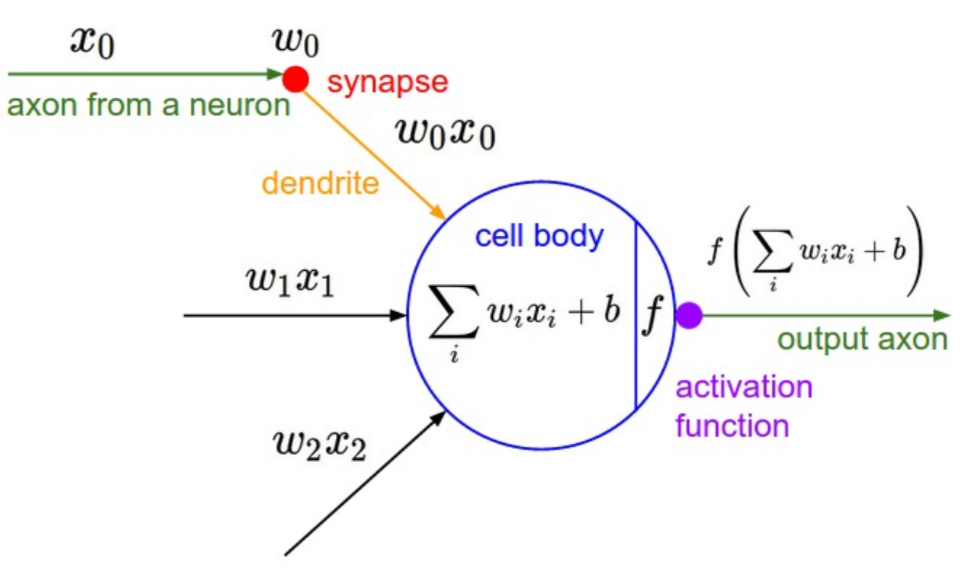
\includegraphics[scale=0.5]{Figs/node.png}
    \caption{A Node}
    \label{node}
\end{figure}

The function $f$ is non-linear and is called the Activation Function. The purpose of the activation function is to introduce non-linearity into the output of a node. The following activation function (Fig.\,\ref{activation}) is often used:
\begin{figure}
	\centering
	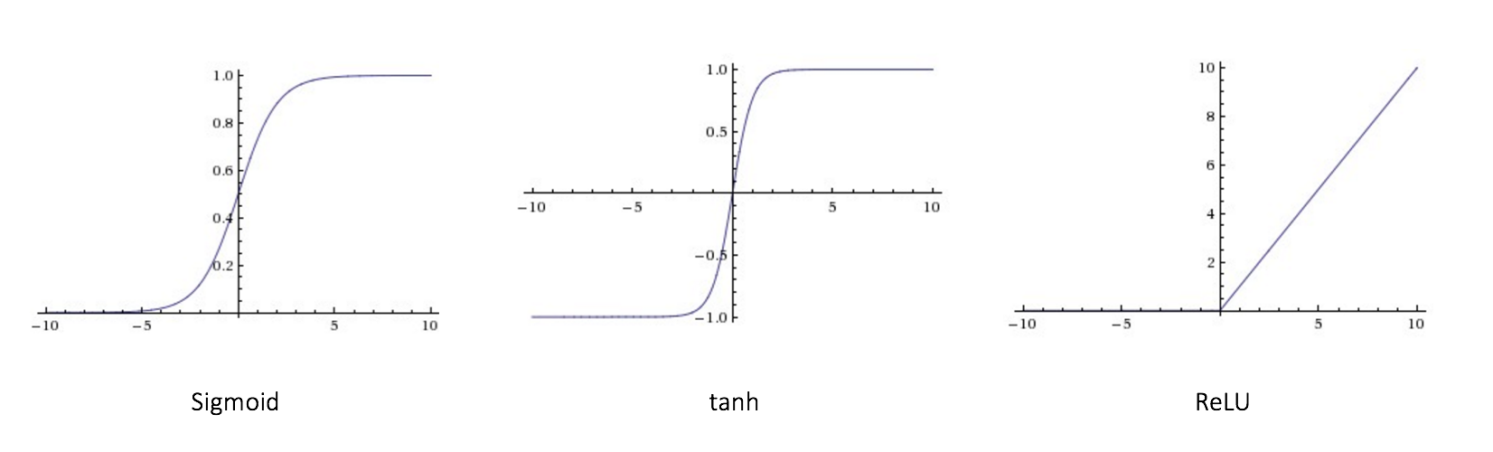
\includegraphics[scale=0.5]{Figs/activation.png}
    \caption{Activation Functions}
    \label{activation}
\end{figure}

\begin{itemize}
  \item Sigmoid: takes a real-valued input and squashes it to range between 0 and 1
        $$ \sigma(x) =  \frac{\mathrm{1} }{\mathrm{1} + e^{-x} }  $$ 
  \item tanh: takes a real-valued input and squashes it to the range [-1, 1]
        $$ tanh(x) = 2\cdot\sigma(2x)-1 $$
        
  \item ReLU(Rectified Linear Unit): takes a real-valued input and thresholds it at zero
        $$f(x) = \max(0,x)$$
\end{itemize}

\subsection{Feedforward Neural Network}

The simplest Neural Network is a feedforward fully connected network. It is formed by one or multiple layers of nodes. Nodes in adjacent layers have connections between them. A connection represents a set of weights.


\noindent An example of a feedforward neural network is shown in Fig.\,\ref{feedforward}.
\begin{figure}[h]
	\centering
	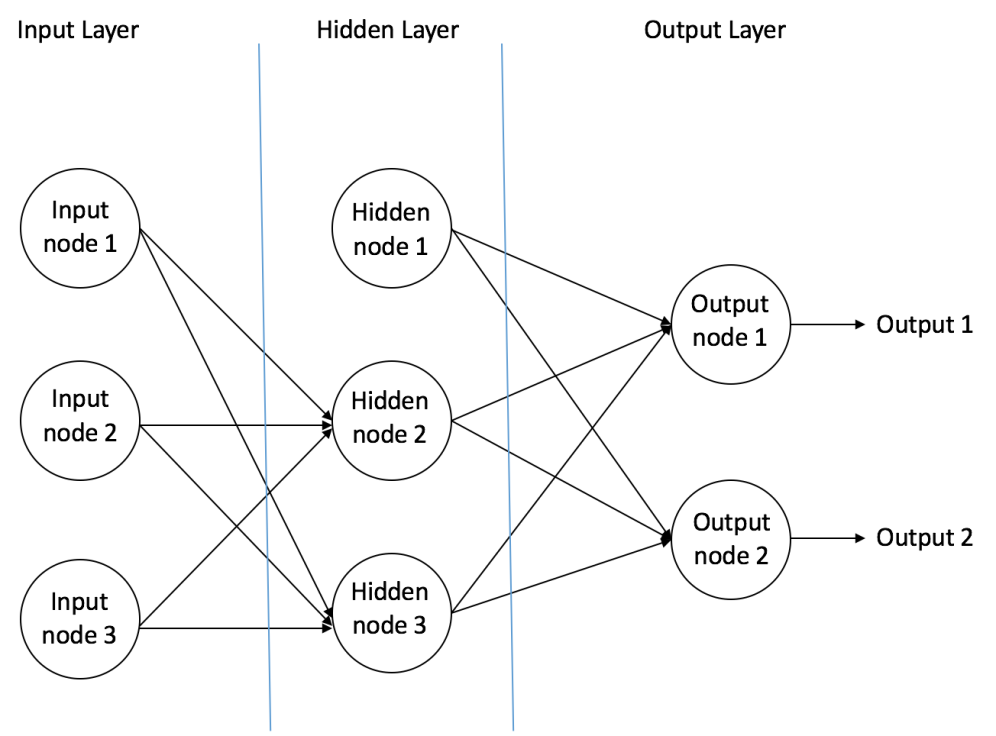
\includegraphics[scale=0.5]{Figs/feedforward.png}
    \caption{Feedforward Neural Network}
    \label{feedforward}
\end{figure}

A feedforward neural network can consist of three types of nodes:

\begin{enumerate}
\item Input Nodes – The Input nodes take in a input $X$ in the form of vector $(x_1,...,x_n)$. These nodes are together referred to as the “Input Layer”. No computation is performed in any of the Input nodes – they just pass on the information to the hidden nodes.

\item Hidden Nodes – The Hidden nodes are in between Input Layer and Output Layer. They have no direct connection with the network input and the network output, thus they are called "Hidden" and form "Hidden Layer". After training, Hidden Node will learn some relationship (non-linearality) between its input and output. A feedforward network can have zero, one, or multiple Hidden Layers.

\item Output Nodes – The Output nodes are collectively referred to as the “Output Layer” and are responsible for computations and producing output from the "Hidden Layer". Output Layer works in similar way as a Hidden Layer, but the output of this layer is considered the final output of the network.

\end{enumerate}

In a feedforward network, the information moves in only one direction – forward – from the input nodes, through the hidden nodes and to the output nodes. There are no cycles or loops in the network.


\subsection{Multi Layer Perceptron}
A Multi Layer Perceptron (MLP) contains one or more hidden layers (apart from one input and one output layer).  While a single layer perceptron can only learn linear functions, a multilayer perceptron can also learn non-linear functions.

Fig.\,\ref{mlp} shows a multilayer perceptron with a single hidden layer. Note that all connections have weights associated with them, but only three weights $(w_1,...,w_n)$ are shown in the figure.

\begin{figure}[h]
	\centering
	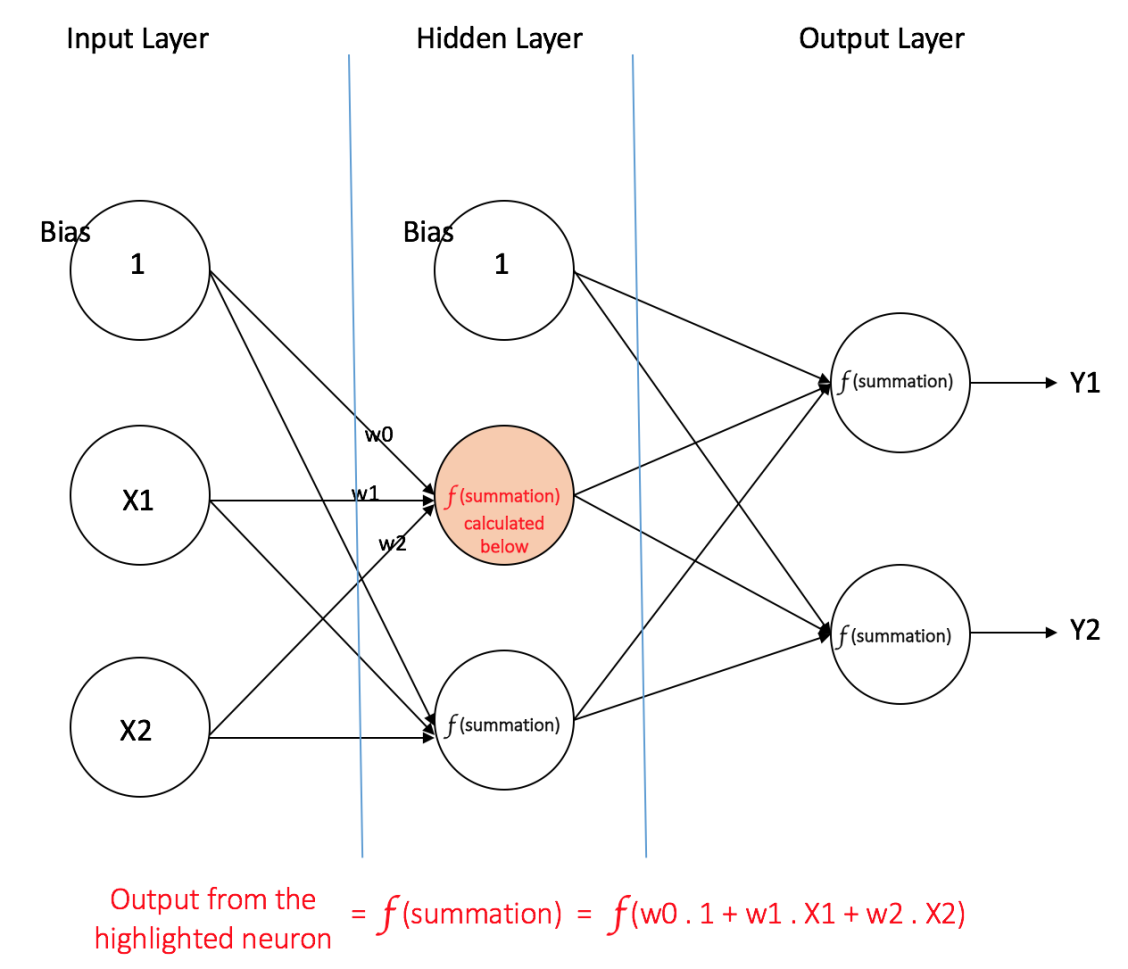
\includegraphics[scale=0.5]{Figs/multilayer.png}
    \caption{Multi Layer Perceptron}
    \label{mlp}
\end{figure}

\textbf{Input Layer}: The Input layer has three nodes. The Bias node has a value of 1. The other two nodes take in the input $X = (x_1,x_2)$. These values form the Input Layer and are passed to the Hidden Layer.

\textbf{Hidden Layer}: The Hidden layer also has three nodes with the Bias node having an output of 1. The output of the other two nodes in the Hidden layer depends on the Input layer $(b, x_1, x_2)$ as well as the weights $(w_0,w_1,...,w_n)$ associated with the connections (edges). Fig.\,\ref{mlp} shows the output calculation for one of the hidden nodes (highlighted). $Y_{Node} = f(\sum{w_0+w_1x_1+w_2x_2})$, where $f$ is an activation function.

\textbf{Output Layer}: The Output layer has two nodes which take inputs from the Hidden layer and perform similar computations as shown for the highlighted hidden node. The values calculated $(y_1,y_2)$ as a result of these computations act as output $\hat{Y}$ of the Multi Layer Perceptron.

Given a set of features $X = (x_1,...,x_n)$ and a target $Y = (y_1,..,y_n)$, a Multi Layer Perceptron can learn the relationship between the features and the target, for either classification or regression.


\subsection{Back-Propagation}
Back-Propagation refers to the backward propagation of errors. A Neural Network learns through Back-Propagation by calculating the error from the output $\hat{Y}$ to the true value $Y$, then improving the weights in all nodes. The learning is "supervised", meaning the true value $Y$ must be given to the network respect to each input $X$ in training.

A loss function $L$ measures the error between network output $\hat{Y}$ and the true value $Y$. The cost of one set of weights is defined as $\mathcal{L}(W)$
$$\mathcal{L}(W)= \frac{\mathrm{1}}{n}\sum_{i=1}^{n} L(Y^i,\hat{Y}^i) = \frac{\mathrm{1}}{n}\sum_{i=1}^{n} L(Y^i,f(X^i,W))$$
Where $Y^i$ are the true values, $X^i$ are the inputs, $\hat{Y}^i$ are the network outputs corresponds to $X^i$. $W$ is the set of weights, and $f$ is the activation function.

There are many loss functions to measure different kind of errors. For a classification problem, which is this project, Cross Entropy loss is used. Cross Entropy is defined as:
$$\mathcal{L}=-\frac{\mathrm{1}}{n}\sum_{i=1}^{n}[Y^i \log(\hat{Y}^i)+(1-Y^i) \log(1-\hat{Y}^i)]$$
measures the divergence between two probability distributions. Minimizing the cross entropy increases the similarities between the two distributions. The use of cross entropy as a loss function is commonly paired with the use of a Sigmoid activation function $\sigma$ when dealing with binary classification. Substituting a Sigmoid activation function $\sigma$
$$\mathcal{L}=-\frac{\mathrm{1}}{n}\sum_{i=1}^{n}[Y^i \log(\sigma(W \cdot X^i))+(1-Y^i) \log(1-\sigma(W \cdot X^i))]$$
The derivative w.r.t weights $W$ is:
$$\frac{\partial \mathcal{L}}{\partial W} = (Y - \sigma(W \cdot X))\cdot X$$
The $\sigma'(W \cdot X)$ term is eliminated, which makes it easy for calculation.
Then the learning is performed by updating W
$$ W = W - \eta\cdot\nabla\mathcal{L}$$
where $\eta$ is a pre-defined learning rate. Often times, the learning rate is difficult to set. If it is too large, the local and global minima can be “overshot”, leading to slow convergence, and if the learning rate is too small, it can take a long time to converge to an acceptable minimum. “Adaptive Moment Estimation (Adam)” optimizer is invented to adaptively set the learning rate during training.


\section{Convolutional Neural Networks}
A Convolutional Neural Network (ConvNet/CNN) is a Neural Network model which can take in an input image, assign importance (learnable weights and biases) to regions/groups of pixels via kernals/filters. The pre-processing required in a ConvNet is much lower as compared to other classification algorithms. While in primitive methods filters are hand-engineered, with enough training, ConvNets have the ability to learn these kernals.

The architecture of a ConvNet is analogous to that of the connectivity pattern of Neurons in the Human Brain and was inspired by the organization of the Visual Cortex. Individual neurons respond to stimuli only in a restricted region of the visual field known as the Receptive Field. A collection of such fields overlap to cover the entire visual area.

\subsection{Convolution Layer — The Kernel}
A ConvNet is able to successfully capture the Spatial and Temporal dependencies in an image through the application of relevant kernels. The architecture performs a better fitting to the image dataset due to the reduction in the number of parameters involved and reusability of weights. In other words, the network can be trained to understand the sophistication of the image better.

An example of kernel could be a simple 3x3 vertical edge detector.

\begingroup
\begin{tabular}{ | *{3}{>{\collectcell\fwcell}c<{\endcollectcell} |} }
  \hline
  1 & 0 & -1 \\
  \hline
  1 & 0 & -1 \\
  \hline
  1 & 0 & -1 \\
  \hline
\end{tabular}}
\endgroup

Let K denote this kernel. Convolution is done by matrix multiplication operation between K and the portion P of the image over which the kernel is hovering. The kernel is moved from left to right, top to bottom with a certain Stride value. Figure * shows two steps of kernal application on image with Stride set to 1. 

ConvNets need not be limited to only one Convolutional Layer. Conventionally, the first ConvLayer is responsible for capturing the Low-Level features such as edges, color, gradient orientation, etc. With added layers, the architecture adapts to the High-Level features as well, giving us a network which has the wholesome understanding of images in the dataset.

\subsection{Pooling Layer}

Similar to the Convolutional Layer, the Pooling layer is responsible for reducing the spatial size of the Convolved Feature. This is to decrease the computational power required to process the data through dimensionality reduction. Furthermore, it is useful for extracting dominant features which are rotational and positional invariant, thus maintaining the process of effectively training of the model.

There are two types of Pooling: Max Pooling and Average Pooling. Max Pooling returns the maximum value from the portion of the image covered by the Kernel. On the other hand, Average Pooling returns the average of all the values from the portion of the image covered by the Kernel.

Max Pooling also performs as a Noise Suppressant. It discards the noisy activations altogether and also performs de-noising along with dimensionality reduction. On the other hand, Average Pooling simply performs dimensionality reduction as a noise suppressing mechanism. Hence, we can say that Max Pooling performs a lot better than Average Pooling.

The Convolutional Layer and the Pooling Layer, together form the i-th layer of a Convolutional Neural Network. Depending on the complexities in the images, the number of such layers may be increased for capturing low-levels details even further, but at the cost of more computational power.

\subsection{Classification — Fully Connected Layer (FC Layer)}

Adding a Fully-Connected layer is a (usually) cheap way of learning non-linear combinations of the high-level features as represented by the output of the convolutional layer. The Fully-Connected layer is learning a possibly non-linear function in that space.

Now that we have converted our input image into a suitable form for our Multi-Level Perceptron, we shall flatten the image into a column vector. The flattened output is fed to a feed-forward neural network and backpropagation applied to every iteration of training. Over a series of epochs, the model is able to distinguish between dominating and certain low-level features in images and classify them using the Softmax Classification technique.

\section{K-Fold Cross Validation}
\section{Image data augmentation}



 
% remember to set these at the start of each chapter
\chapter{CNN Architecture} 
\label{arcgutecture} 

%%%%%%%%%%%%%%%%%%
\section{VGG}
\section{ResNet}
\section{Small CNN}

% remember to set these at the start of each chapter
\chapter{Experiments and Discussion} 
\label{experiments}
In this section, we show and discuss the performance of each of the CNN models: Small CNN, VGG, VGG-IN, and ResNet. The training is performed on the US and PAT datasets and two other datasets for verification. Section \ref{result_dataset} and \ref{result_aug} describe the US and PAT datasets and data pre-processing. Section \ref{result_training} describes the training process, and Section \ref{result_curves} and \ref{result_acc} include experimental results. We then have a discussion about the results in Section \ref{result_discussion}. Finally, the experimental results on the other two datasets are shown in Section \ref{result_other}.
%%%%%%%%%%%%%%%%%%
\section{Dataset}
\label{result_dataset}
The dataset is obtained from the study of \cite{Kosik2019}. It contains 90 breast cancer tumour samples, each of which has an Ultrasound (US) image stack and a Photoacoustic (PAT) image stack. In the dataset, each sample belongs to one of 14 types (class A - N) of cancer, where the actual cancer name is masked to obtain a blind study. The distribution of cancer classes is shown in Fig.\,\ref{class_graph}.  
\begin{figure}[h]
	\centering
	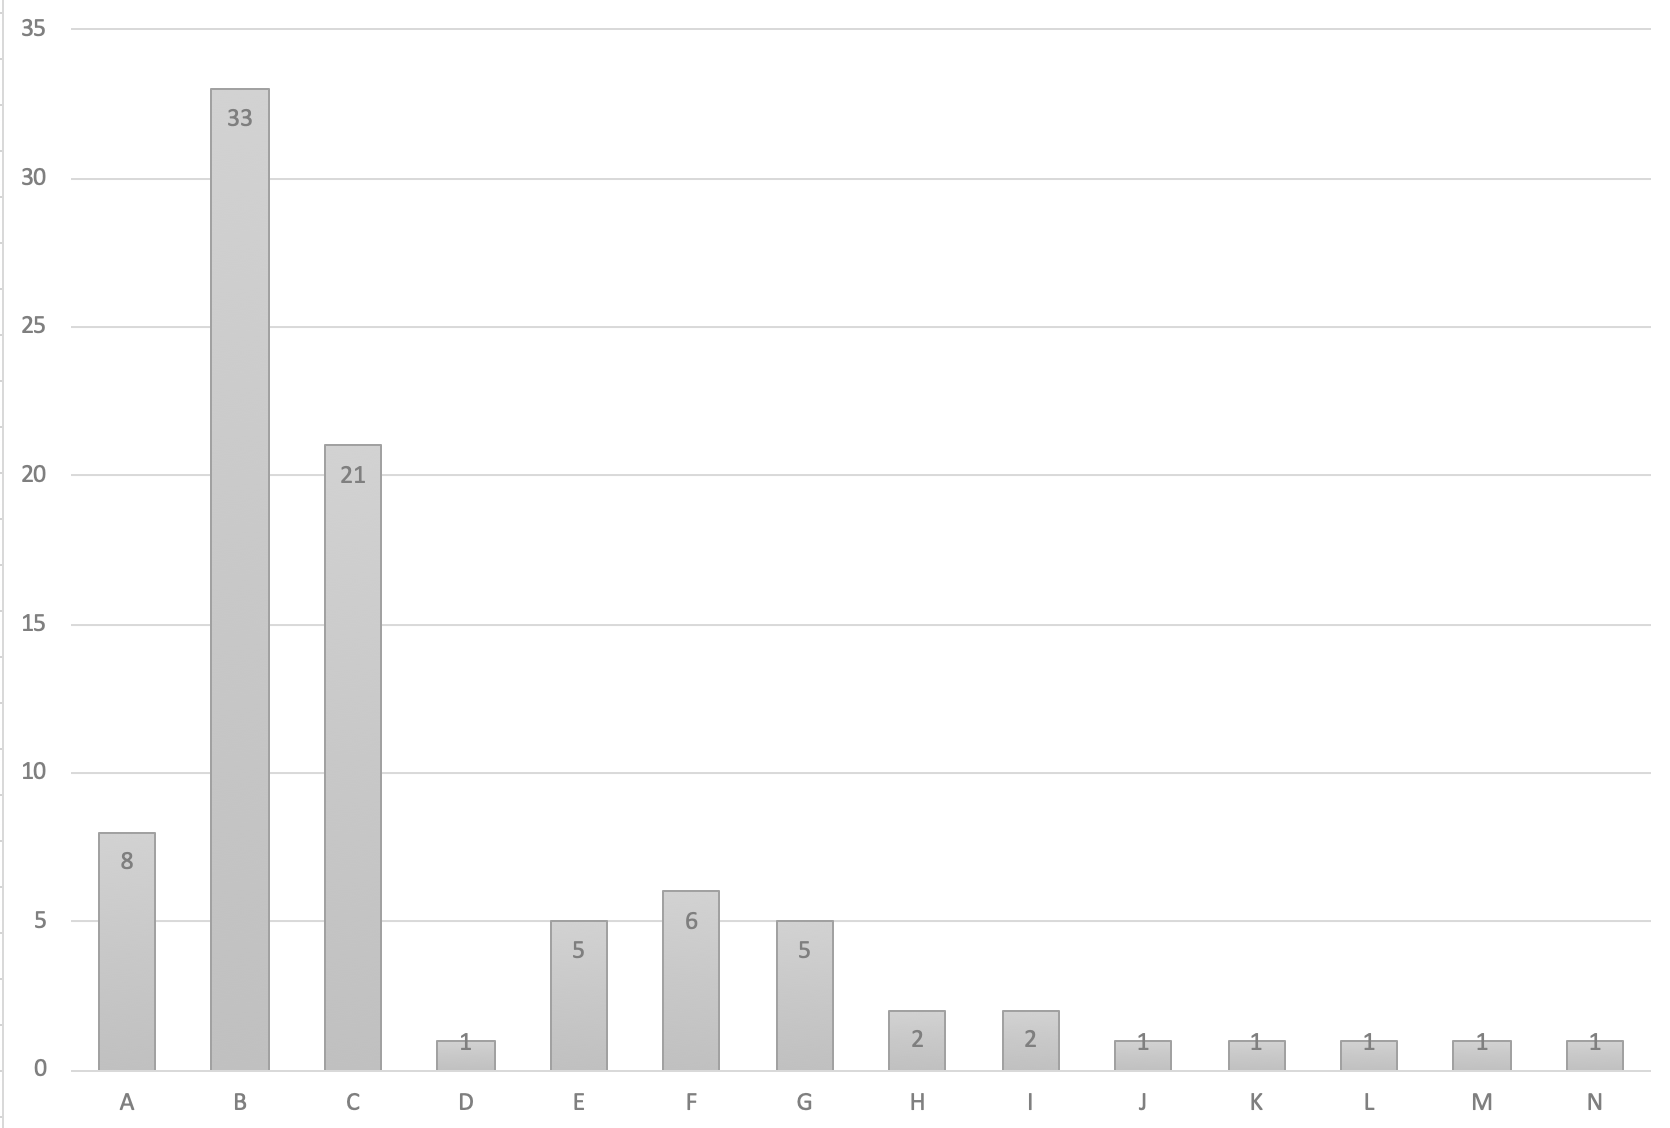
\includegraphics[width=0.7\textwidth]{Figs/class_graph.png}
    \caption{Cancer types and number of samples per type}
    \label{class_graph}
\end{figure}

B has 33 samples and C has 21 samples. In this project, only class B and C are used, because the other classes have too few samples to train a neural network.

A specimen of breast cancer tumour is scanned in the $z$ direction (vertical) relative to the holding platform. Scans produce a stack of 2D images of the cross-section. An example of an image stack is shown in Fig.\,\ref{stack}. 

\begin{figure}[h]
	\centering
	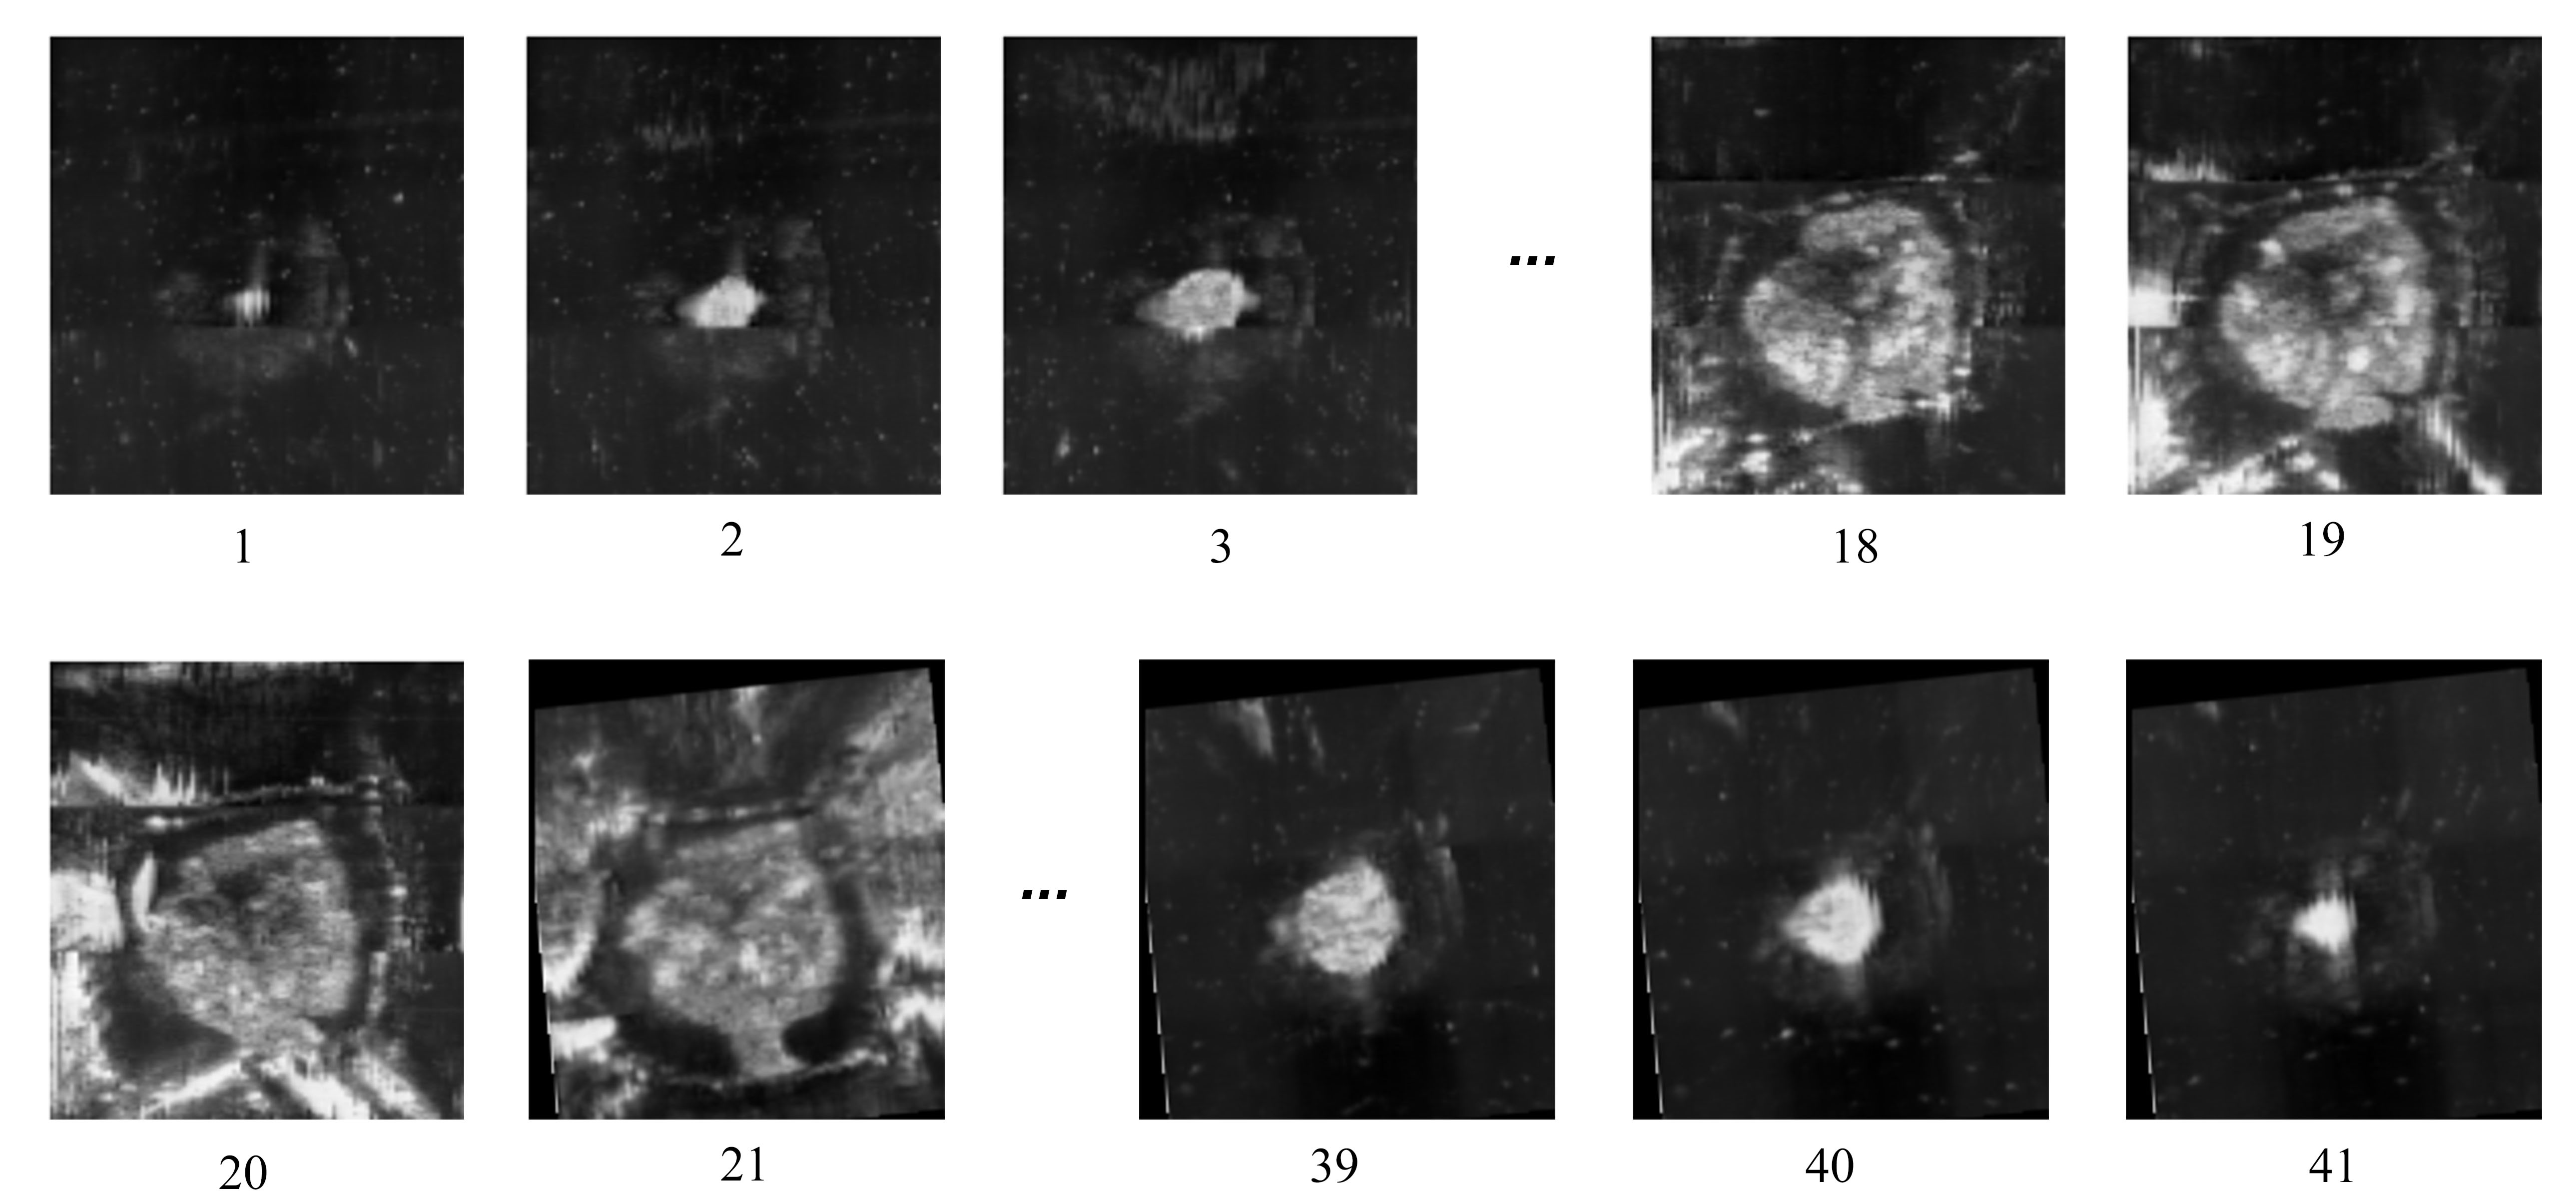
\includegraphics[width=\textwidth]{Figs/pat_stack_50.jpg}
    \caption{US stack example}
    \label{stack}
\end{figure}

We can see that the top and bottom scans, for example 1, 2, 3, 39, 40, 41 in Fig.\,\ref{stack}, are very small and lack detail for the internal texture. This is because the cross-sections close to the top and bottom of a tumour specimen are very small. The cross-sections close to the centre of a specimen, such as 18, 19, 21, 21 are larger in size and have more texture. For each image stack, US and PAT, the centre 6 images are extracted to use for training and validation (we could extract more or even use all of the images, but we may not want to use images with poor quality). There are in total 389 PAT images and 344 US images extracted from the stacks. Examples of such images are shown in Fig.\,\ref{pat_us_example}.

\begin{figure}
\centering
\begin{subfigure}[b]{.24\linewidth}
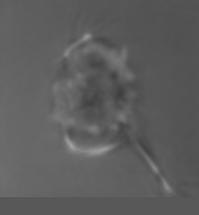
\includegraphics[width=\linewidth]{Figs/PAT014_18.jpg}
\caption{AF014 PAT}
\end{subfigure}
\begin{subfigure}[b]{.24\linewidth}
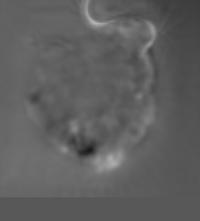
\includegraphics[width=\linewidth]{Figs/PAT023_23.jpg}
\caption{AF023 PAT}
\end{subfigure}
\begin{subfigure}[b]{.24\linewidth}
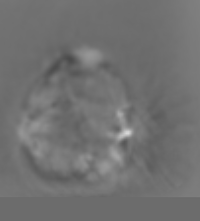
\includegraphics[width=\linewidth]{Figs/PAT36.png}
\caption{AF036 PAT}
\end{subfigure}
\begin{subfigure}[b]{.24\linewidth}
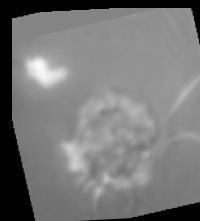
\includegraphics[width=\linewidth]{Figs/PAT055_11.jpg}
\caption{AF055 PAT}
\end{subfigure}

\begin{subfigure}[b]{.24\linewidth}
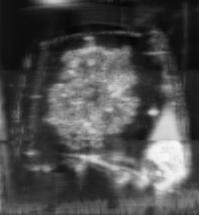
\includegraphics[width=\linewidth]{Figs/US14_18.jpg}
\caption{AF014 US}
\end{subfigure}
\begin{subfigure}[b]{.24\linewidth}
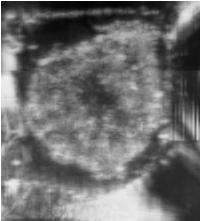
\includegraphics[width=\linewidth]{Figs/US23_23.jpg}
\caption{AF023 US}
\end{subfigure}
\begin{subfigure}[b]{.24\linewidth}
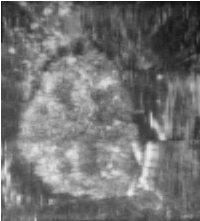
\includegraphics[width=\linewidth]{Figs/US36.png}
\caption{AF036 US}
\end{subfigure}
\begin{subfigure}[b]{.24\linewidth}
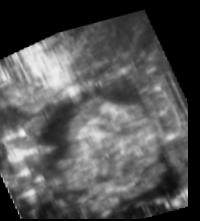
\includegraphics[width=\linewidth]{Figs/US55_13.jpg}
\caption{AF055 US}
\end{subfigure}
\caption{Extracted PAT and US images}
\label{pat_us_example}
\end{figure}

\section{Data Partition and Augmentation}
\label{result_aug}

The images are divided into a training set and a testing set by an 80/20 ratio. No image from the same stack is present in both the training and the testing sets. Because the number of samples in class B and C is not balanced, a K-fold data partitioning is done using a stratified k-fold. A stratified K-fold is where the training set and the testing set contain approximately the same percentage of samples of each target class as the original dataset. Each of the five folds is used as a test set only once. Accuracy and $F_1$ score (defined in (\ref{f1_score})) are averaged across the five folds.

Machine learning generally requires large amounts of data. Since our dataset is small, data augmentation is used to artificially expand the number of samples. Augmentation Scaling Factor is set to 5, meaning five images are created from one by rotation, cropping, horizontal and vertical flip. Then, the images are resized to (192, 192).

\section{Training}
\label{result_training}

The four CNN models, Small CNN, VGG, VGG-IN, and ResNet are implemented and trained using the open-source neural-network library Keras \citep{chollet2015keras} in Python \citep{van1995python}. The Adam \citep{adam} optimizer is used in all models to minimize the loss function. Adam can adaptively adjust its parameters based on the average first moment, as well as the average of the second moments of the gradients. Initially, the parameters of Adam are set to their defaults. The number of epoch is 50, as all samples are passed to the network 50 times, with a batch size of 32. Checkpoints are used so that the best set of weights is saved. For a classification problem, the loss function is the categorical cross-entropy loss \citep{Goodfellow-et-al-2016}, which is defined as $$-\sum^M_{c=1} y_{o,c}\log(p_{o,c}),$$
where $M$ is the number of classes, $y$ is a binary indicator (0 or 1) if class label $c$ is the correct classification for observation $o$, and $p$ is the predicted probability observation $o$ is of class $c$. 

Training a neural network is a ccomputationally intensive task. To speed up the training process, the program is run on a supercomputer system SHARCNET \citep{sharcnet}.

\section{Accuracy and $F_1$ score}
\label{result_acc}

The $F_1$ score (also called F-score) is a measure of a test's accuracy \citep{powers2011evaluation}. It considers both the precision $p$ and the recall $r$ of the test to compute the score. The $F_1$ score is the harmonic average of the precision and recall, where an $F_1$ score reaches its best value at 1 (perfect precision and recall) and worst at 0.
Formally: 
\begin{equation}\label{f1_score}
    F_1 = 2 \cdot \frac{\mathrm{precision} \cdot \mathrm{recall}}{\mathrm{precision} + \mathrm{recall}} = 2 \cdot \frac{p \cdot r}{p+r},
\end{equation}
where the precision is $$p = \frac{TP}{TP + FP},$$
and the recall is $$r = \frac{TP}{TP + FN}.$$
\noindent Here TP denotes the number of true positives: outcomes where the model correctly predicts the positive class.

\noindent TN denotes the number of true negatives: outcomes where the model correctly predicts the negative class.

\noindent FP denotes the number of false positives: outcomes where the model incorrectly predicts the positive class.

\noindent FN denotes the number of false negatives: outcomes where the model incorrectly predicts the negative class.

\begin{table}[h]
\centering
\begin{tabular}{ |p{4cm}||p{3cm}|p{3cm}|p{3cm}|  }
 \hline
 Model       & Accuracy & Class B $F_1$ score & Class C $F_1$ score\\
 \hline
 \hline
 Small  US   & 0.66  & 0.77 &  0.23\\
 ResNet US   & \textbf{0.75}  & \textbf{0.82} &  \textbf{0.55}\\
 VGG US      & 0.61  & 0.76 &  0\\
 VGG-IN US & 0.65 & 0.77 & 0.22 \\
\hline
 Small PAT   & 0.71  & 0.79 &  0.50\\
 ResNet PAT  & 0.76  & 0.83 &  \textbf{0.57}\\
 VGG PAT     & 0.61  & 0.76 &  0\\
 VGG-IN PAT & \textbf{0.78} & \textbf{0.84} & 0.54 \\
 \hline
\end{tabular}
\caption{Model accuracy and $F_1$ score on the US and PAT datasets}
\label{acctable}
\end{table}

\section{Training Curves}
\label{result_curves}
\label{section_curves}

\begin{figure}
\centering
\begin{subfigure}[b]{.45\linewidth}
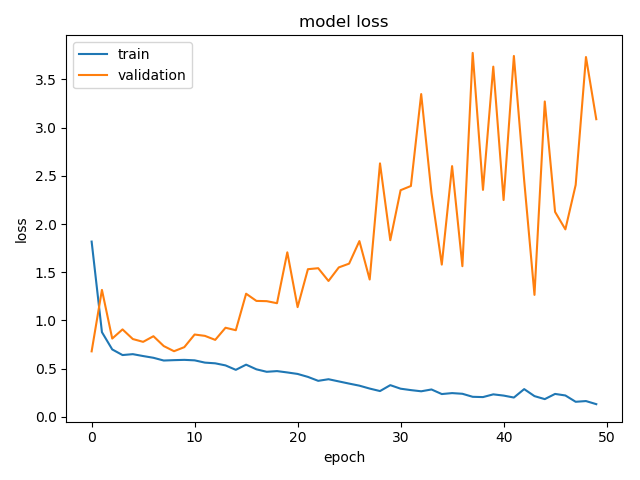
\includegraphics[width=\linewidth]{Figs/small_us_loss.jpg}
\caption{Small CNN US}
\end{subfigure}
\begin{subfigure}[b]{.45\linewidth}
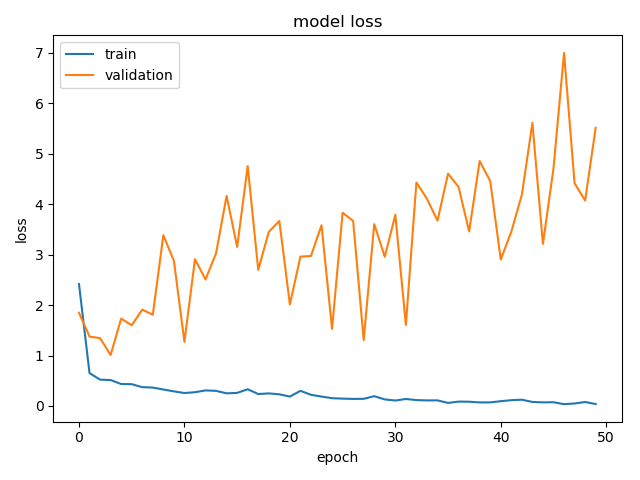
\includegraphics[width=\linewidth]{Figs/small_pat_loss.jpg}
\caption{Small CNN PAT}
\end{subfigure}

\begin{subfigure}[b]{.45\linewidth}
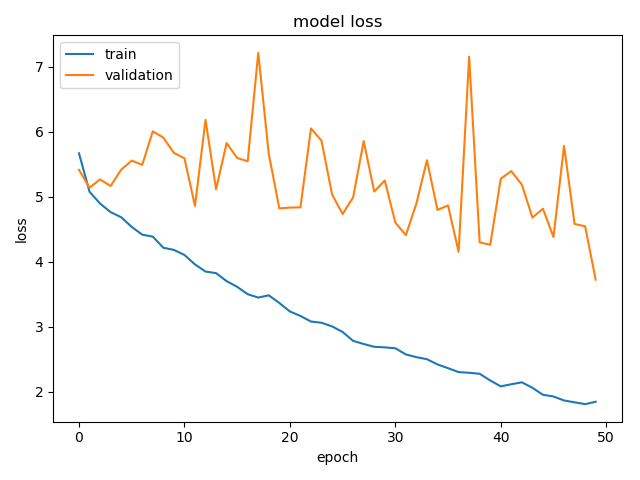
\includegraphics[width=\linewidth]{Figs/resnet_us_loss.jpg}
\caption{ResNet US}
\end{subfigure}
\begin{subfigure}[b]{.45\linewidth}
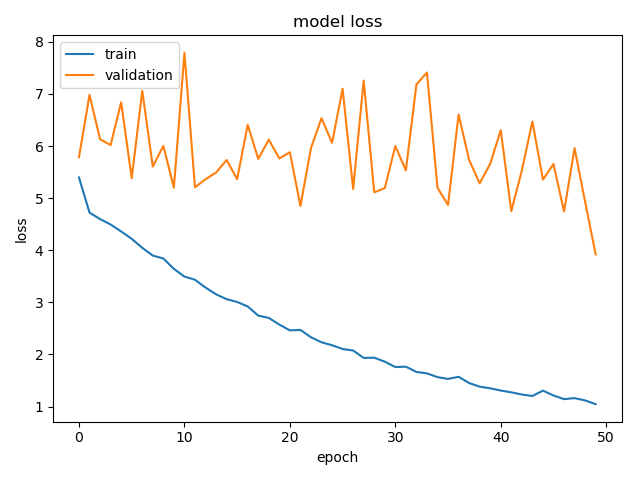
\includegraphics[width=\linewidth]{Figs/resnet_pat_loss.jpg}
\caption{ResNet PAT}
\end{subfigure}

\begin{subfigure}[b]{.45\linewidth}
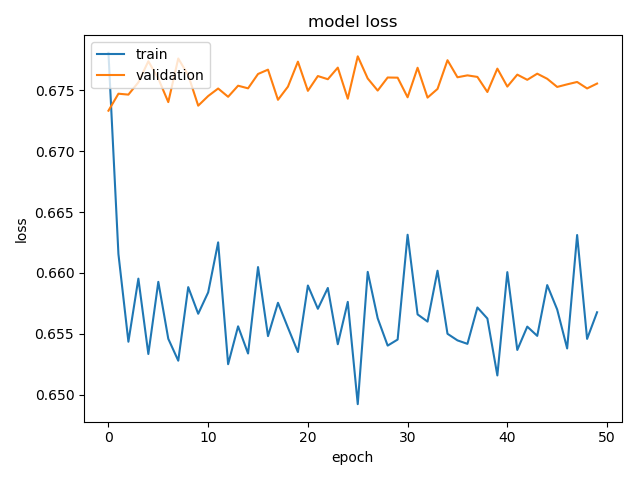
\includegraphics[width=\linewidth]{Figs/vgg_us_loss.jpg}
\caption{VGG US}
\end{subfigure}
\begin{subfigure}[b]{.45\linewidth}
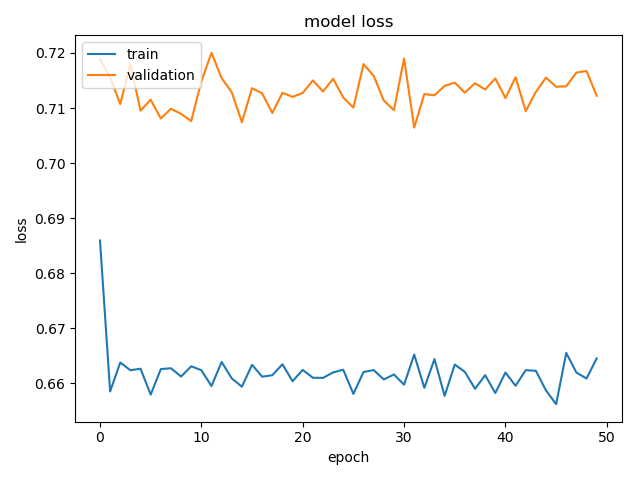
\includegraphics[width=\linewidth]{Figs/vgg_pat_loss.jpg}
\caption{VGG PAT}
\end{subfigure}

\begin{subfigure}[b]{.45\linewidth}
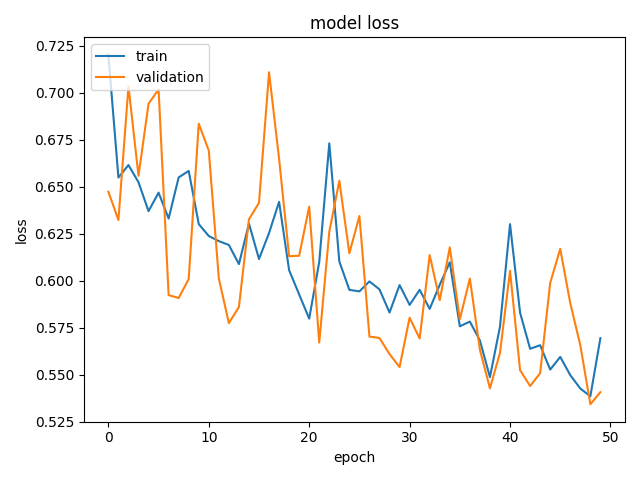
\includegraphics[width=\linewidth]{Figs/vgg_in_us_loss.jpg}
\caption{VGG-IN US}
\end{subfigure}
\begin{subfigure}[b]{.45\linewidth}
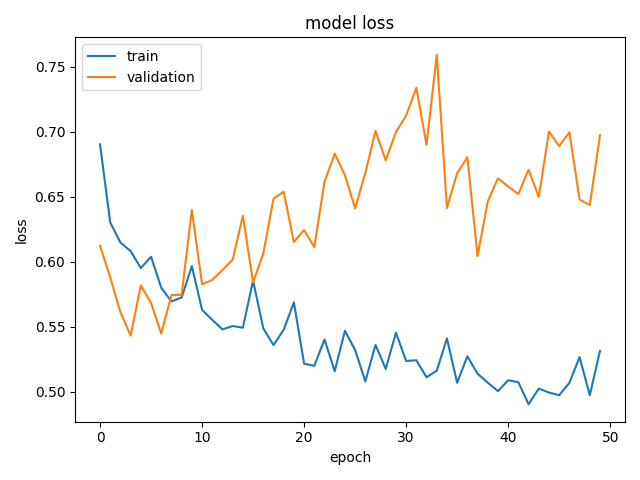
\includegraphics[width=\linewidth]{Figs/vgg_in_pat_loss.jpg}
\caption{VGG-IN PAT}
\end{subfigure}
\caption{Model loss on the US and PAT datasets}
\label{fig:loss}
\end{figure}

\begin{figure}
\centering
\begin{subfigure}[b]{.45\linewidth}
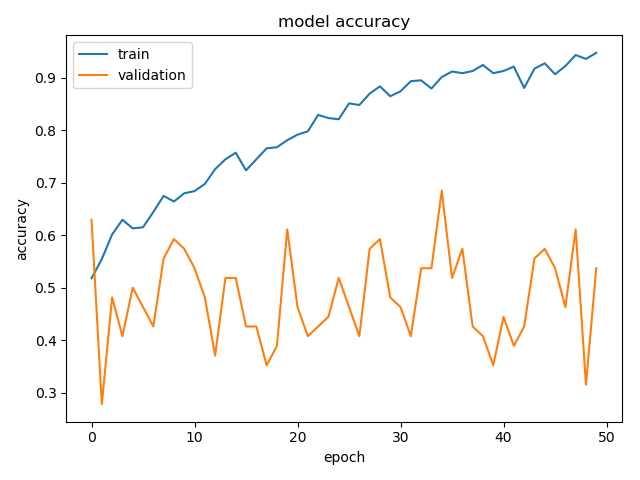
\includegraphics[width=\linewidth]{Figs/small_us_acc.jpg}
\caption{Small CNN US}
\end{subfigure}
\begin{subfigure}[b]{.45\linewidth}
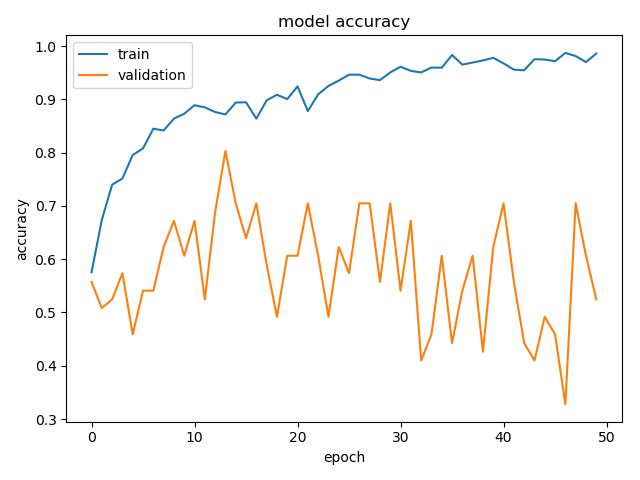
\includegraphics[width=\linewidth]{Figs/small_pat_acc.jpg}
\caption{Small CNN PAT}
\end{subfigure}

\begin{subfigure}[b]{.45\linewidth}
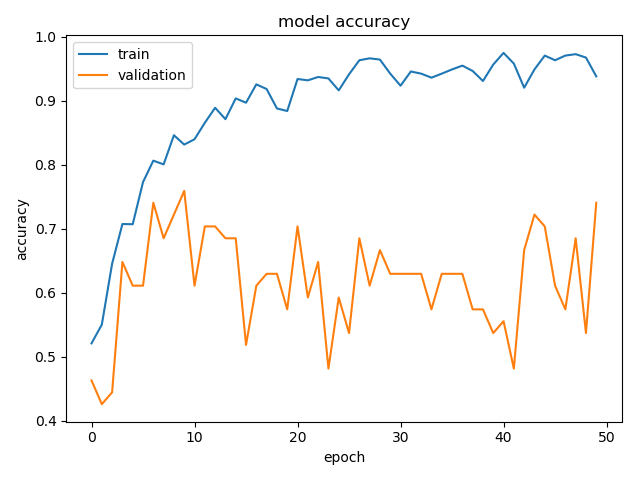
\includegraphics[width=\linewidth]{Figs/resnet_us_acc.jpg}
\caption{ResNet US}
\end{subfigure}
\begin{subfigure}[b]{.45\linewidth}
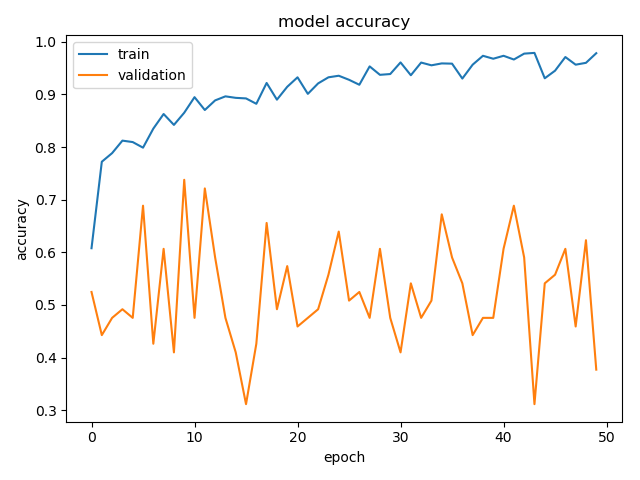
\includegraphics[width=\linewidth]{Figs/resnet_pat_acc.jpg}
\caption{ResNet PAT}
\end{subfigure}

\begin{subfigure}[b]{.45\linewidth}
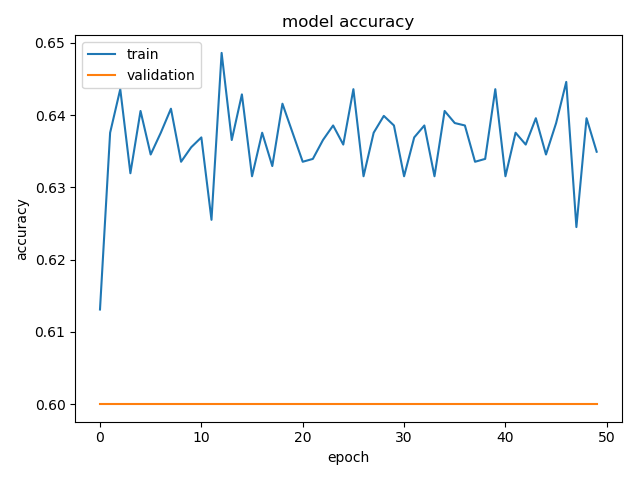
\includegraphics[width=\linewidth]{Figs/vgg_us_acc.jpg}
\caption{VGG US}
\end{subfigure}
\begin{subfigure}[b]{.45\linewidth}
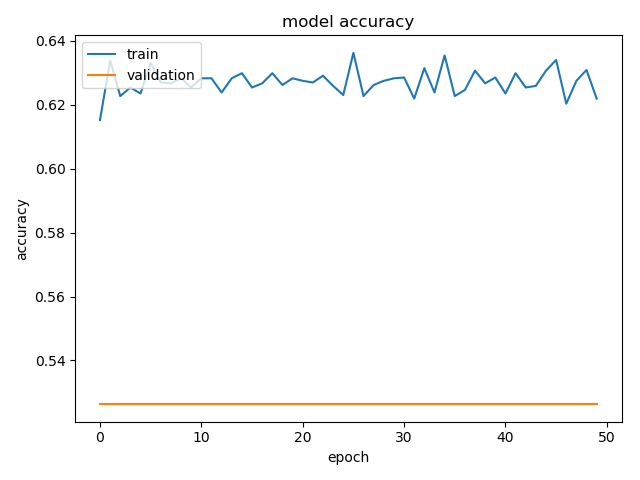
\includegraphics[width=\linewidth]{Figs/vgg_pat_acc.jpg}
\caption{VGG PAT}
\end{subfigure}

\begin{subfigure}[b]{.45\linewidth}
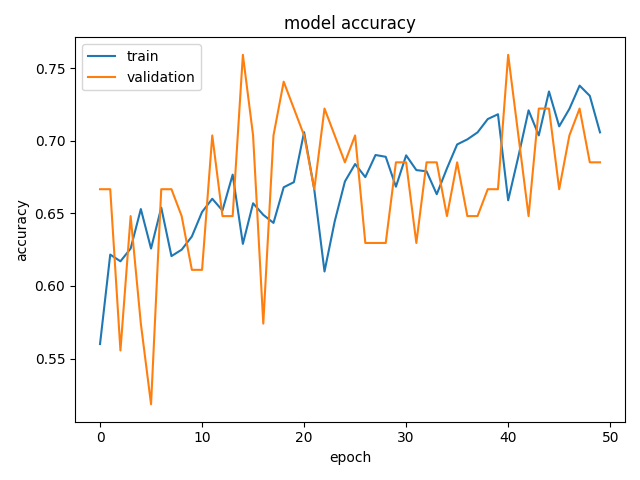
\includegraphics[width=\linewidth]{Figs/vgg_in_us_acc.jpg}
\caption{VGG-IN US}
\end{subfigure}
\begin{subfigure}[b]{.45\linewidth}
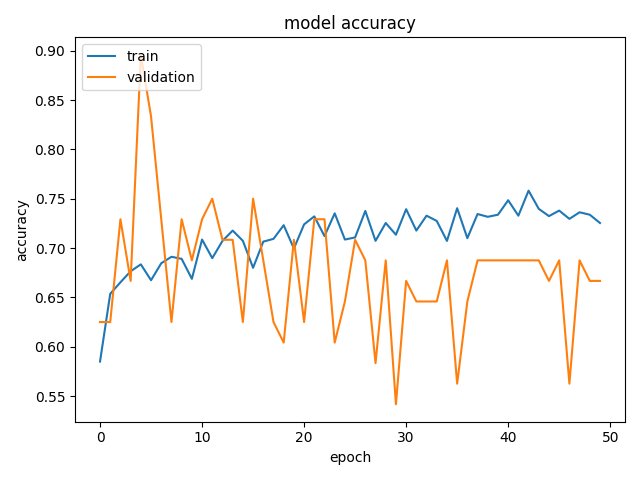
\includegraphics[width=\linewidth]{Figs/vgg_in_pat_acc.jpg}
\caption{VGG-IN PAT}
\end{subfigure}
\caption{Model accuracy on the US and PAT datasets}
\label{fig:acc}
\end{figure}

The learning process of a neural network can be investigated through training curves \citep{Anzanello2011}. Training and validation loss and accuracy are reported and ploted in Fig.\,\ref{fig:loss} and Fig.\,\ref{fig:acc}. 


\section{Discussion}
\label{result_discussion}

For the Small CNN model, even though the training loss is decreasing, the validation loss is increasing (Fig.\,\ref{fig:loss} (A) (B)). This model is not generalizing to fit unseen validation data. For the ResNet model, the decrease of the training and validation loss (Fig.\,\ref{fig:loss} (C) (D)) indicates that ResNet could improve from training (although very noisy). The VGG model has almost the same depth as ResNet, 19 layers versus 18 layers. Yet, the convergence of the training and validation loss is poor. We do not see a decrease in the training and validation loss (Fig.\,\ref{fig:loss} (E) (F)). The VGG-IN model uses a set of pre-trained weights from the ImageNet \citep{imagenet_cvpr09} in the convolutional layers, and only the fully-connected layers and classification layer are trained. The VGG-IN model shows decrease in training and validation loss on the US dataset (Fig.\,\ref{fig:loss}), but on the PAT dataset (Fig.\,\ref{fig:loss} (H)) only the training loss decreases.

All models perform poorly in terms of accuracy on the US and PAT datasets. The validation accuracy of all models do not show a consistent improvement over the epochs (Fig.\,\ref{fig:acc}). Note the large gap between the training and validation curves. This indicates that the training dataset is unrepresentative, which means that the training dataset does not provide sufficient information to learn. We may have too few examples in the training dataset, or the training dataset may not be a good representation. From the noisy validation curves, we can conclude that the validation dataset is also unrepresentative. A unrepresentative validation set means that it does not provide sufficient information to evaluate the ability of the model to generalize. This could occur when the validation dataset has too few examples.

Medical images are naturally difficult to acquire. By machine learning standards, which often requires thousands or even millions of samples, our datasets is considered extremely small. In addition, the US and and in particular the PAT scans are very noisy and have many artifacts. The low quality of images makes it more challenging for the neural networks to pick up important features. If more data is available, we hope to see an improvement on the models' performance.

\section{Experiments with other datasets}
\label{result_other}

\begin{figure}[h]
\centering
\begin{subfigure}[b]{.2\linewidth}
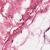
\includegraphics[width=\linewidth]{Figs/8864_idx5_x1251_y1651_class0.png}
\end{subfigure}
\begin{subfigure}[b]{.2\linewidth}
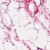
\includegraphics[width=\linewidth]{Figs/8864_idx5_x1201_y1801_class0.png}
\end{subfigure}
\begin{subfigure}[b]{.2\linewidth}
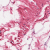
\includegraphics[width=\linewidth]{Figs/8864_idx5_x1201_y1701_class0.png}
\end{subfigure}
\begin{subfigure}[b]{.2\linewidth}
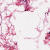
\includegraphics[width=\linewidth]{Figs/8864_idx5_x1151_y1701_class0.png}
\end{subfigure}

\begin{subfigure}[b]{.2\linewidth}

\includegraphics[width=\linewidth]{Figs/8864_idx5_x1851_y2251_class1.png}
\end{subfigure}
\begin{subfigure}[b]{.2\linewidth}
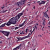
\includegraphics[width=\linewidth]{Figs/8864_idx5_x1801_y2701_class1.png}
\end{subfigure}
\begin{subfigure}[b]{.2\linewidth}
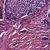
\includegraphics[width=\linewidth]{Figs/8864_idx5_x1801_y2651_class1.png}
\end{subfigure}
\begin{subfigure}[b]{.2\linewidth}
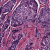
\includegraphics[width=\linewidth]{Figs/8864_idx5_x1801_y2551_class1.png}
\end{subfigure}
\caption{Examples from the IDC Breast Cancer dataset}
\label{IDC}
\end{figure}

\begin{figure}[h]
\centering
\begin{subfigure}[b]{.2\linewidth}
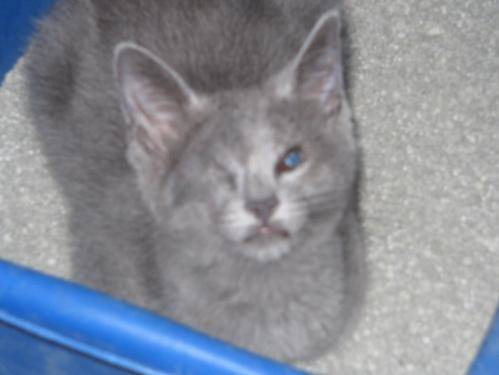
\includegraphics[width=\linewidth]{Figs/cat450.jpg}
\end{subfigure}
\begin{subfigure}[b]{.2\linewidth}
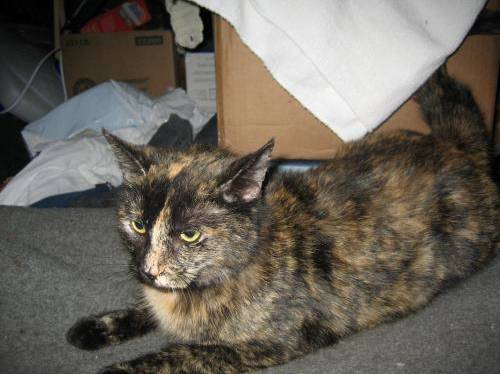
\includegraphics[width=\linewidth]{Figs/cat1921.jpg}
\end{subfigure}
\begin{subfigure}[b]{.2\linewidth}
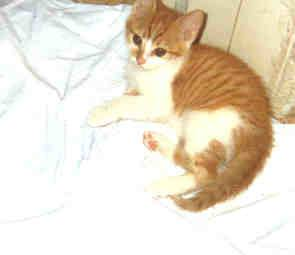
\includegraphics[width=\linewidth]{Figs/cat1412.jpg}
\end{subfigure}
\begin{subfigure}[b]{.2\linewidth}
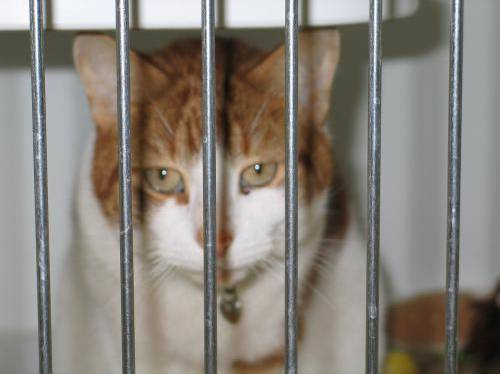
\includegraphics[width=\linewidth]{Figs/cat1168.jpg}
\end{subfigure}

\begin{subfigure}[b]{.2\linewidth}
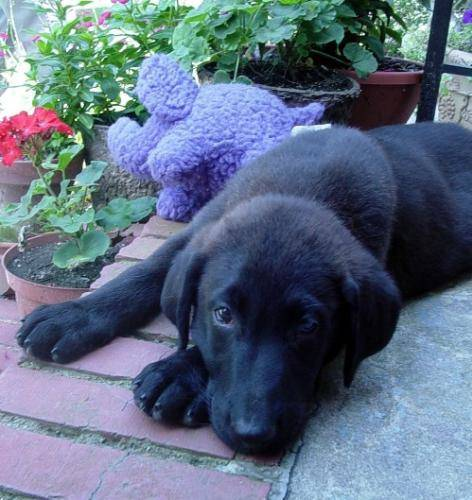
\includegraphics[width=\linewidth]{Figs/dog876.jpg}
\end{subfigure}
\begin{subfigure}[b]{.2\linewidth}
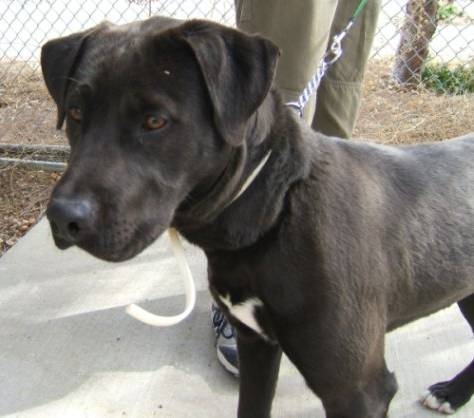
\includegraphics[width=\linewidth]{Figs/dog508.jpg}
\end{subfigure}
\begin{subfigure}[b]{.2\linewidth}
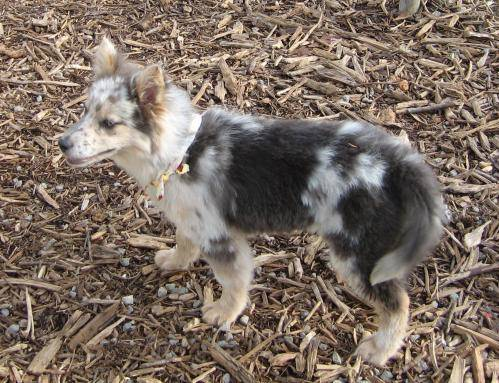
\includegraphics[width=\linewidth]{Figs/dog4133.jpg}
\end{subfigure}
\begin{subfigure}[b]{.2\linewidth}
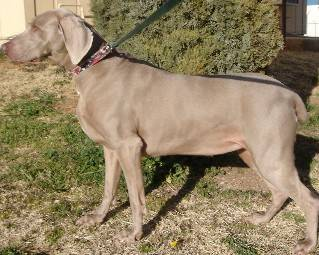
\includegraphics[width=\linewidth]{Figs/dog1178.jpg}
\end{subfigure}
\caption{Examples from the Cats vs. Dogs dataset}
\label{catdog}
\end{figure}

Due to the poor performance on our US and PAT datasets, to verify the capabilities of these neural network models, we trained them on two other classification datasets, the IDC Breast Cancer dataset \citep{Janowczyk2016} (Fig.\,\ref{IDC}) and the Dogs vs. Cats dataset \citep{catdog}  (Fig.\,\ref{catdog}).


Table \ref{stats} shows the number of images in the datasets. The models are trained for 10 epoch on the IDC Breast Cancer Dataset and 30 epoch on the Dogs vs. Cats Dataset.
\begin{table}[h]
\centering
\begin{tabular}{ |p{3cm}||p{3cm}|p{3cm}|  }
 \hline
 Class       & Training set & Validation set\\
 \hline
 \hline
 IDC class 0   & 179,343   &  68,549 \\
 IDC class 1  & 71,609  & 27,763\\
 \hline
 Cat   & 10,499  &  2,003\\
 Dog  & 10,499  &  2,003\\
 \hline
\end{tabular}
\caption{Number of images in each set}
\label{stats}
\end{table}


\begin{table}[h]
\centering
\begin{tabular}{ |p{4cm}||p{3cm}|p{3cm}|p{3cm}|  }
 \hline
 Model       & Accuracy & Class 0 $F_1$ score & Class 1 $F_1$ score\\
 \hline
 \hline
 Small IDC Breast   & \textbf{0.89}  & \textbf{0.92} &  \textbf{0.80}\\
 ResNet IDC Breast  & 0.88  & \textbf{0.92} &  \textbf{0.80}\\
 VGG IDC Breast      & 0.71  & 0.83 &  0\\
 VGG-IN IDC Breast & 0.85 & 0.90 & 0.73 \\
 \hline
 Small CatDog   & \textbf{0.93}  & \textbf{0.93} &  \textbf{0.93}\\
 ResNet CatDog  & \textbf{0.93}  & \textbf{0.93} &  \textbf{0.93}\\
 VGG CatDog      & 0.50  & 0.67 &  0\\
 VGG-IN CatDog  & 0.92 & 0.92 & 0.92 \\
  \hline
\end{tabular}
\caption{Model accuracy and $F_1$ score on the IDC Breast Cancer dataset and the Dogs vs. Cats dataset}
\label{acctable2}
\end{table}

Validation accuracy and $F_1$ score are reported in Table \ref{acctable2}. The Small CNN model and the ResNet model achieved about the same accuracy and $F_1$ score on both datasets. The VGG model did not training well. Using pre-trained weights in the VGG-IN model is effective to improve the VGG model, but the performance still does not match the Small CNN and the ResNet models. A deep neural network model such as VGG is very difficult to train due to the degradation problem. A deep network not necessarily performs better than a shallower network.

Training loss and accuracy plots are shown in Fig.\,\ref{fig:loss2}. 

\begin{figure}[h]
\centering
\begin{subfigure}[b]{.45\linewidth}
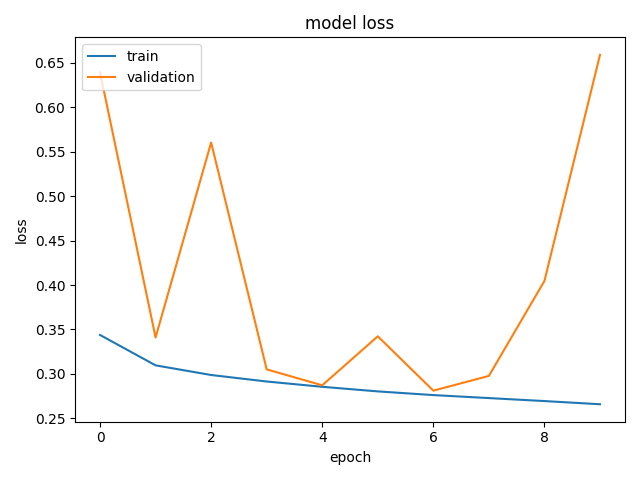
\includegraphics[width=\linewidth]{Figs/small_breast_loss.jpg}
\caption{Small IDC Breast}
\end{subfigure}
\begin{subfigure}[b]{.45\linewidth}
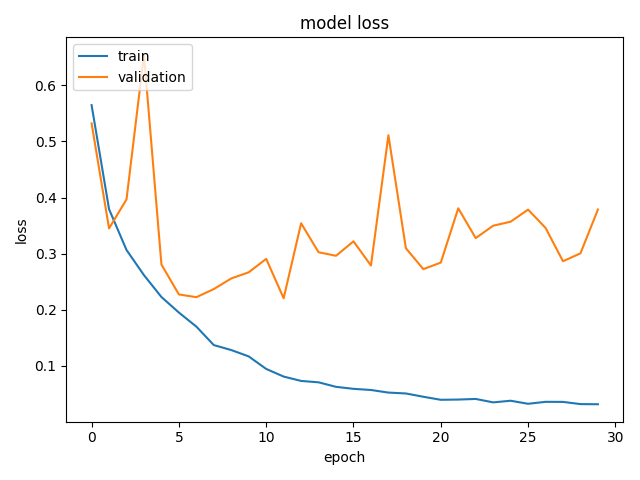
\includegraphics[width=\linewidth]{Figs/small_catdog_loss.jpg}
\caption{Small CatDog}
\end{subfigure}

\begin{subfigure}[b]{.45\linewidth}
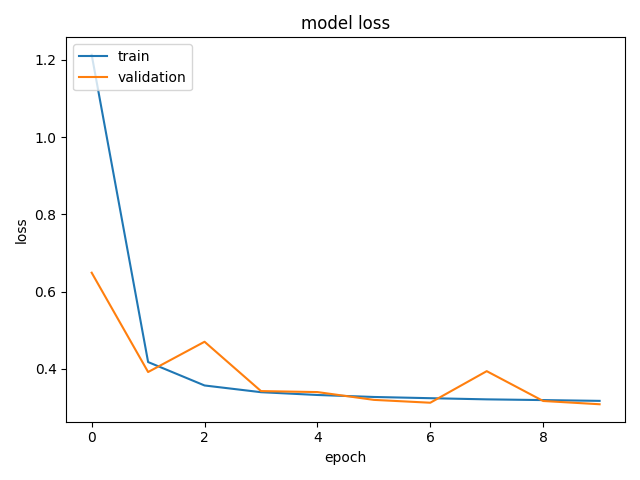
\includegraphics[width=\linewidth]{Figs/resnet_breast_loss.jpg}
\caption{ResNet IDC Breast}
\end{subfigure}
\begin{subfigure}[b]{.45\linewidth}
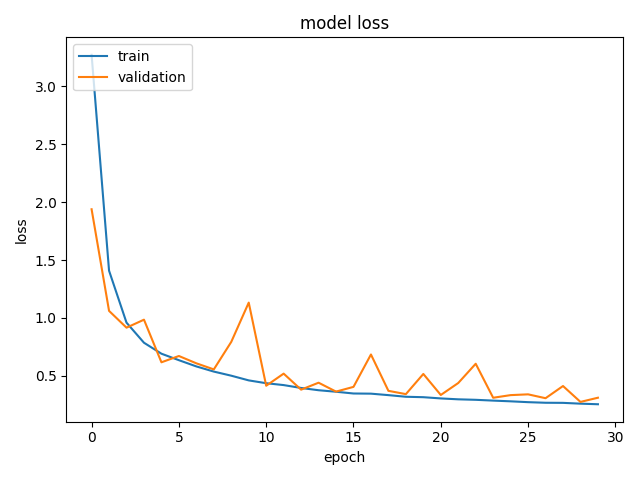
\includegraphics[width=\linewidth]{Figs/resnet_catdog_loss.jpg}
\caption{ResNet CatDog}
\end{subfigure}

\begin{subfigure}[b]{.45\linewidth}
\includegraphics[width=\linewidth]{Figs/vgg_breast_loss.jpg}
\caption{VGG IDC Breast}
\end{subfigure}
\begin{subfigure}[b]{.45\linewidth}
\includegraphics[width=\linewidth]{Figs/vgg_catdog_loss.jpg}
\caption{VGG CatDog}
\end{subfigure}

\begin{subfigure}[b]{.45\linewidth}
\includegraphics[width=\linewidth]{Figs/vgg_in_breast_loss.jpg}
\caption{VGG-IN IDC Breast}
\end{subfigure}
\begin{subfigure}[b]{.45\linewidth}
\includegraphics[width=\linewidth]{Figs/vgg_in_catdog_loss.jpg}
\caption{VGG-IN CatDog}
\end{subfigure}

\caption{Model loss on the IDC Breast Cancer dataset and the Dogs vs. Cats dataset}
\label{fig:loss2}
\end{figure}

\begin{figure}
\centering
\begin{subfigure}[b]{.45\linewidth}
\includegraphics[width=\linewidth]{Figs/small_breast_acc.jpg}
\caption{Small IDC Breast}
\end{subfigure}
\begin{subfigure}[b]{.45\linewidth}
\includegraphics[width=\linewidth]{Figs/small_catdog_acc.jpg}
\caption{Small CatDog}
\end{subfigure}

\begin{subfigure}[b]{.45\linewidth}
\includegraphics[width=\linewidth]{Figs/resnet_breast_acc.jpg}
\caption{ResNet IDC Breast}
\end{subfigure}
\begin{subfigure}[b]{.45\linewidth}
\includegraphics[width=\linewidth]{Figs/resnet_catdog_acc.jpg}
\caption{ResNet CatDog}
\end{subfigure}

\begin{subfigure}[b]{.45\linewidth}
\includegraphics[width=\linewidth]{Figs/vgg_breast_acc.jpg}
\caption{VGG IDC Breast}
\end{subfigure}
\begin{subfigure}[b]{.45\linewidth}
\includegraphics[width=\linewidth]{Figs/vgg_catdog_acc.jpg}
\caption{VGG CatDog}
\end{subfigure}

\begin{subfigure}[b]{.45\linewidth}
\includegraphics[width=\linewidth]{Figs/vgg_in_breast_acc.jpg}
\caption{VGG-IN IDC Breast}
\end{subfigure}
\begin{subfigure}[b]{.45\linewidth}
\includegraphics[width=\linewidth]{Figs/vgg_in_catdog_acc.jpg}
\caption{VGG-IN CatDog}
\end{subfigure}

\caption{Model accuracy on the IDC Breast Cancer dataset and the Dogs vs. Cats dataset}
\label{fig:acc2}
\end{figure}


% I suggest only compiling one chapter at a time, and comment out the others. That way, the document will typeset faster. When your done with all the chapters, then uncomment them all. Don't worry about the numbering of chapters/figures/etc. LaTeX will take care of that. 

%----------------------------------------------------------------------------------------
%	THESIS CONTENT - APPENDICES
%----------------------------------------------------------------------------------------

\appendix % Cue to tell LaTeX that the following "chapters" are Appendices
\renewcommand{\thetable}{A\arabic{chapter}.\arabic{table}} % adds an A to table names in appendix (Table A1.1, A1.2...)
\renewcommand{\thefigure}{A\arabic{chapter}.\arabic{figure}} % same for figures
\renewcommand{\thesection}{A\arabic{section}}

% Include the appendices of the thesis as separate files from the Appendices folder
\chapter{Chapter 1 Supplement} % Main appendix title

\label{Supp_chap1}

Here is the supplemental file for chapter 1, as an alternative to including it in the main \TeX for chapter 1. This allows the figures/table to be numbered in a different way and for the section to be listed in the table of contents differently. 


\begin{figure}[h] % put figure roughly here, will float though
	\centering
	\includegraphics[scale=0.4]{Figs/Wright_1932_1.pdf}
    \caption[Same Fig]{Same fig as before, but in the appendix!}
    \label{Another_fig}
\end{figure}


%----------------------------------------------------------------------------------------
%	BIBLIOGRAPHY
%----------------------------------------------------------------------------------------

\printbibliography[heading=bibintoc]

%----------------------------------------------------------------------------------------

\end{document}